%File: features.tex
%Date: Mon Dec 30 19:25:01 2013 +0800
%Author: Yuxin Wu <ppwwyyxxc@gmail.com>


\section{Features}
\subsection{MFCC}
\begin{frame}[label=mfcc]{MFCC}
  \textbf{Mel-Frequency Cepstral Coefficients}

  Cepstral feature which closely approximates human auditory system's response.
  Commonly used feature for Speech/Speaker Recognition.
\begin{center}
  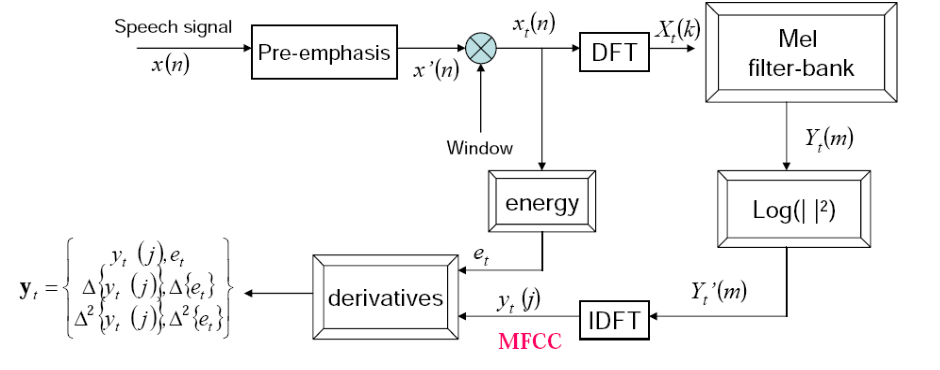
\includegraphics[width=\textwidth]{res/MFCC.png}
\end{center}
\end{frame}

\begin{frame}{Windowing}
\begin{center}
  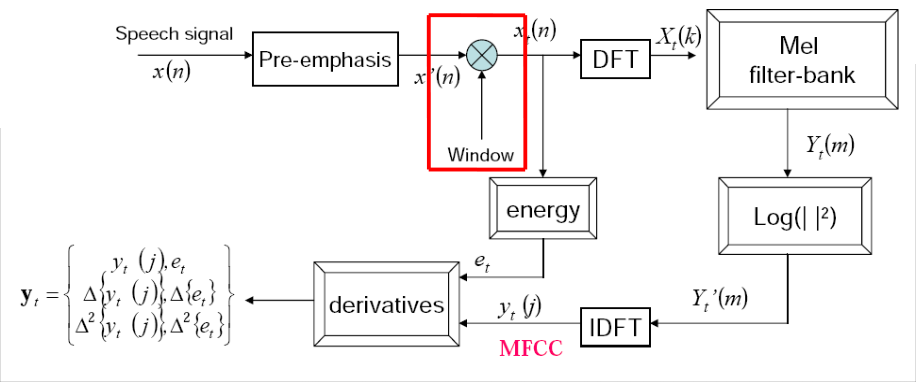
\includegraphics[width=0.6\textwidth]{res/MFCC-windowing.png}\\
  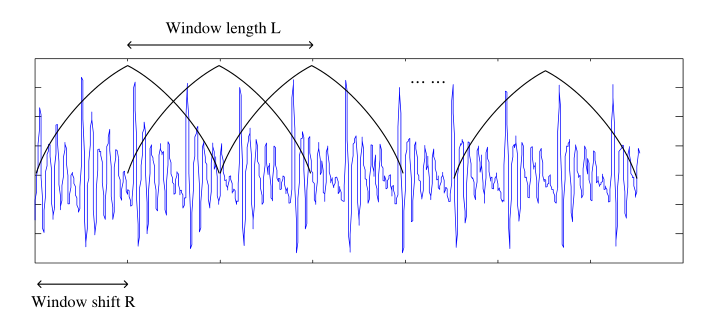
\includegraphics[width=0.8\textwidth]{res/MFCC-windowing-frames.png}
\end{center}
\end{frame}

\begin{frame}{Mel-Scale}
\begin{center}
  \includegraphics[width=0.6\textwidth]{res/MFCC-mel-filterbank.png}
\end{center}
\begin{columns}
  \begin{column}{0.5\textwidth}
    \[ Mel(f) = 2595 \log_{10}(1 + \dfrac{f}{700})\]
  \end{column}
  \begin{column}{0.5\textwidth}
    \begin{flushleft}
      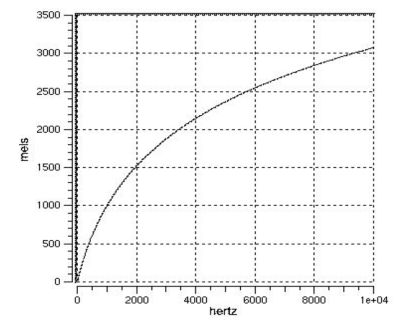
\includegraphics[width=0.7\textwidth]{res/mel-scale.png}
    \end{flushleft}
  \end{column}
\end{columns}
\end{frame}
\againframe{mfcc}


\subsection{LPC}
\begin{frame}{LPC}
  \textbf{Linear Predictive Coding/Coefficients}

\begin{exampleblock}{Assumption}
    In a short period, the $n$th signal is a linear combination of previous $p$ signals:
    $ \hat{x}(n) = \sum_{i=1}^pa_i x(n-i)$
\end{exampleblock}
\pause
Minimize squared error $\text{E}\left[ \hat{x}(n) - x(n)\right] $ using Levinson-Durbin algorithm.

Use $a_1, \cdots  , a_p$ as features.
\end{frame}

\subsection{Experiments on Features}
\begin{frame}{MFCC Params}
\begin{columns}[t]
  \begin{column}[t]{0.5\textwidth}
    \begin{center}
    \includegraphics[width=0.8\textwidth]{res/mfcc-nceps.pdf}\\
    \includegraphics[width=0.8\textwidth]{res/mfcc-frame-len.pdf}
  \end{center}
  \end{column}
  \begin{column}[t]{0.5\textwidth}
    \begin{center}
    \includegraphics[width=0.8\textwidth]{res/mfcc-nfilter.pdf}\\
    Best parameters in our cases:

    Number of cepstrals: 15

    Number of filters: 55

    Frame length: 32ms
  \end{center}
  \end{column}
\end{columns}
\end{frame}

\begin{frame}{LPC Params}
  \begin{center}
    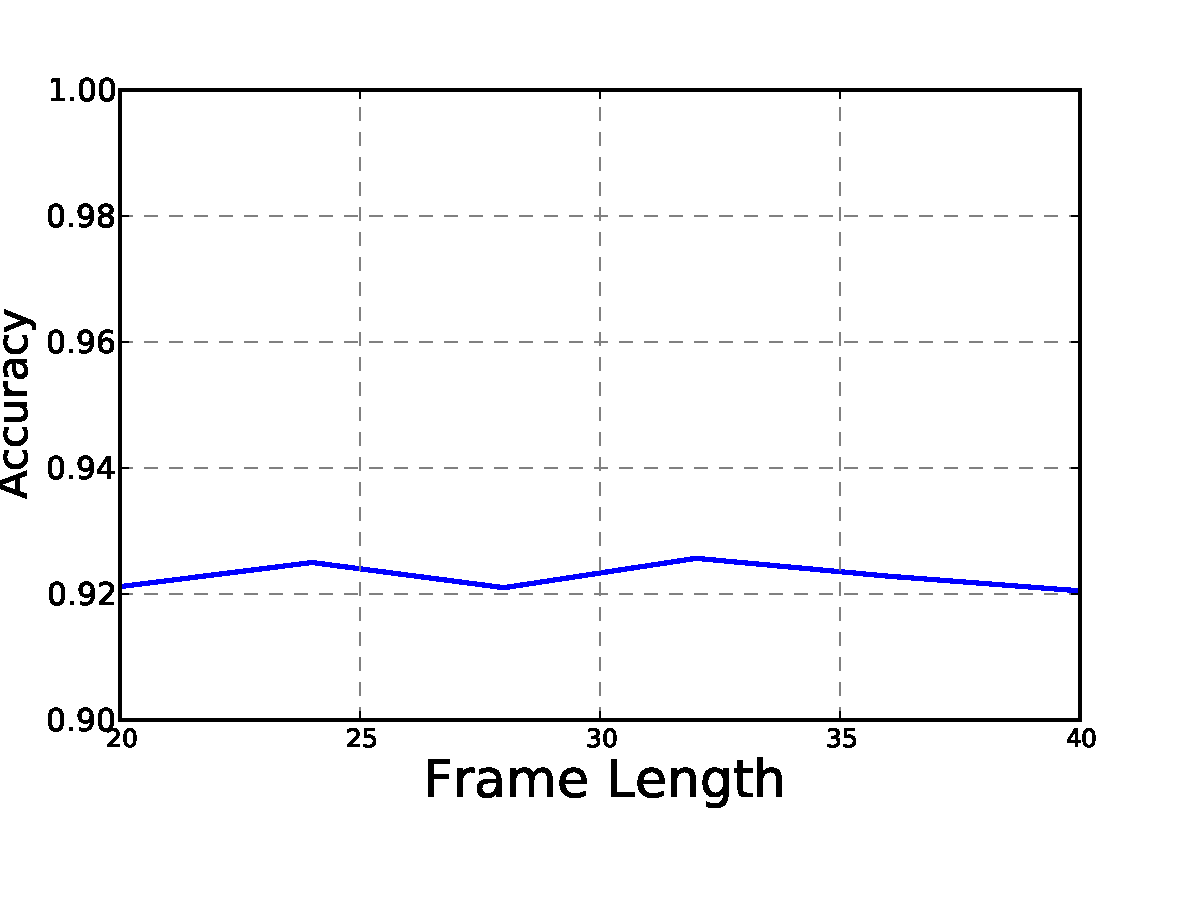
\includegraphics[width=0.5\textwidth]{res/lpc-frame-len.pdf}
    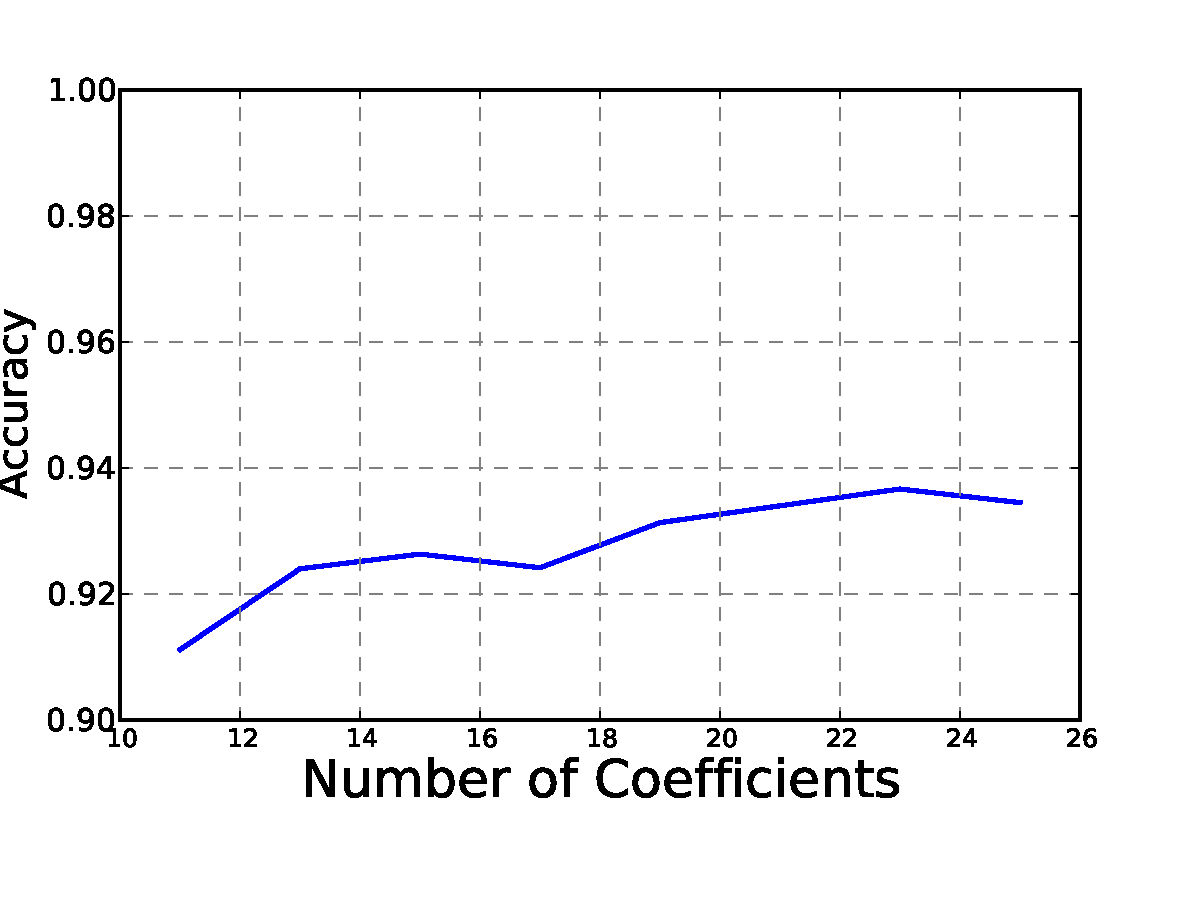
\includegraphics[width=0.5\textwidth]{res/lpc-nceps.pdf}\\
    Best parameter in our cases:

    Number of coefficients: 23

    Frame length: 32ms
  \end{center}
\end{frame}
